\chapter{相关理论基础}
本章对论文中所涉及到的相关理论基础进行了介绍。首先介绍了注意力机制与Transformer模型架构,其次对Transformer模型在图表示学习领域中的应用进行了概述,最后对不同类型的知识图谱嵌入方法的核心思想和数学公式进行了说明,包括传统的知识图谱嵌入方法、基于图神经网络的知识图谱嵌入方法、基于图路径的知识图谱嵌入方法以及基于Transformer的知识图谱嵌入方法。

\section{注意力机制与Transformer网络}
深度学习中的注意力机制(Attention Mechanism)灵感来源于人类的视觉和认知系统。在推理过程中,注意力机制动态的为输入数据分配不同的权重,使模型能够自动地学习并选择性地关注输入中的重要信息,提高模型的性能和泛化能力。注意力机制最早被用于处理计算机视觉任务,后来在多个领域中得到了应用,例如自然语言处理和推荐系统等。

谷歌的研究团队于2017年提出的Transformer网络则是注意力机制方面里程碑式的工作。Transformer网络设计之初主要用于处理序列数据,在Transformer出现之前,序列数据的处理通常依赖于循环神经网络(RNN)及其变体,例如长短期记忆网络(LSTM)和门控递归单元(GRU)。RNN及其变体在处理序列数据时能够保持一定程度的历史信息,但存在一定的问题:由于对序列数据进行逐步处理,RNN在训练过程中容易出现梯度消失或者梯度爆炸的问题,特别是在处理长序列时;逐步处理也限制了模型的并行计算能力,导致训练效率低下;此外,尽管LSTM和GRU通过特殊的门控机制改善了长距离依赖问题,但当序列长度过高时,模型依然难以捕捉到距离较远的依赖关系。

Transformer网络通过使用自注意力(Self-Attention)机制解决了上述问题,在自注意力机制中,输入数据中的任意一个位置都能够直接感知到其它位置的信息,因此相比于传统的RNN结构,自注意力能够更加直接地捕捉到序列中长距离的依赖关系;自注意力机制允许模型在处理数据时并行计算各个位置的注意力分数,与RNN逐步计算的方式相比,可以显著提高模型的计算效率;自注意力机制通过学习输入序列中不同位置之间的动态相关性,能够根据特定的任务自适应地调整注意力分布。

Transformer网络中的自注意力机制的核心为缩放点积注意力机制,结构如图\ref{DotProductAttention}所示。
\begin{figure}[htbp]
  \centerline{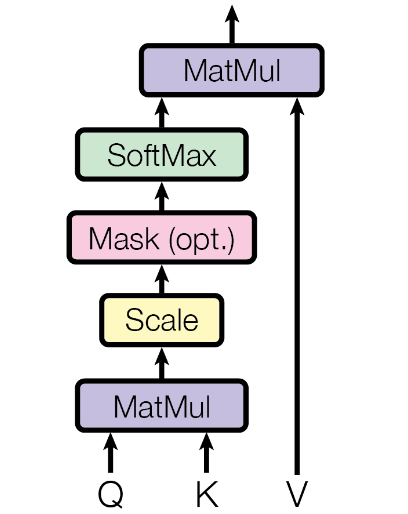
\includegraphics[width=0.30\textwidth]{pic/DotProductAttention.png}}
  \caption{缩放点积注意力机制}
  \label{DotProductAttention}
\end{figure}

具体来说,假设模型的输入为$X$,首先模型将会通过线性变化生成输入对应的查询向量$Q$,键向量$K$以及值向量$V$:
\begin{gather}
    Q=XW^Q, K=XW^K, V=XW^K
\end{gather}
其中$W^Q$、$W^K$、$W^K$是可学习的参数矩阵。

随后模型会将查询向量$Q$和键向量$K$进行点积并乘以缩放因子$\frac{1}{\sqrt{d_k}}$获得注意力分数,将其进行归一化处理转化为概率分布,用作权重对值向量$V$进行加权平均和,最终得到缩放点积注意力机制对应的输出,其中$d_k$为键向量的维度:
\begin{gather}
    \mbox{Attention}(Q,K,V) = \mbox{softmax}(\frac{QK^T}{\sqrt{d_k}})V
\end{gather}


进一步的,为了让模型能够同时关注来自不同维度的信息,并稳定自注意力的学习过程,Transformer采用了多头注意力机制,通过不同的参数矩阵将$Q$、$K$、$V$映射到不同的向量空间下并计算缩放点积注意力,将结果进行拼接获得最终的输出,如图\ref{MultiHeadAttention}所示。

具体来说,对于$h$个独立的注意力头,有:
\begin{equation}
  \begin{aligned}
    \mbox{MultiHead}(Q,K,V)&=\mbox{Concat}(head_1,...,head_h)W^O\\
    \mbox{where} \  head_i &=\mbox{Attention}(QW^Q_i,KW^K_i,VW^V_i)
  \end{aligned}
\end{equation}
其中$QW^Q_i$、$KW^K_i$、$VW^V_i$为将$Q$、$K$、$V$映射到第$i$个向量空间的参数矩阵,Concat为拼接操作。

\begin{figure}[htbp]
  \centerline{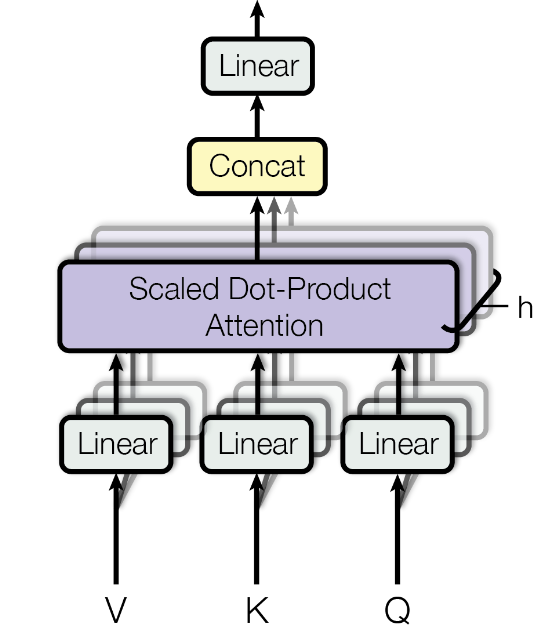
\includegraphics[width=0.4\textwidth]{pic/MultiHeadAttention.png}}
  \caption{多头注意力机制}
  \label{MultiHeadAttention}
\end{figure}
\section{基于Transformer的图表示学习方法}

\section{知识图谱嵌入方法}

\subsection{传统的知识图谱嵌入方法}

\subsection{基于图神经网络的知识图谱嵌入方法}

\subsection{基于图路径的知识图谱嵌入方法}

\subsection{基于Transformer的知识图谱嵌入方法}